

\section{Deterministic inference collapses diverse reasoning paths into a single brittle trace}
\label{sec:reasoning-collapse}

So far, we have focused on \emph{what} deterministic inference hides.
On GLUE--style classification, greedy decoding yields deceptively sharp
point estimates that \emph{look} stable but crumble under paraphrases
and perturbations.
On style-- and constraint--satisfying summarization, it anchors models
to a narrow corner of the semantic--constraint surface, masking the
latent probability mass assigned to instruction--compliant outputs.
We now turn to a third axis: \textbf{multi--step reasoning}.

For reasoning, the question is not only whether a model produces the
\emph{right answer}, but \emph{how many distinct ways it knows to get
there}.
Complex problems often admit several valid solution paths and a rich
spectrum of near--miss failures.
Under \textbf{strict greedy decoding}, however, an LLM's conditional
distribution $p_\theta(\tau \mid x)$ over full chains of thought is
collapsed to a single winning trace
$\tau^{\mathrm{greedy}}(x)$---a \textbf{single, brittle trajectory}
through a much larger space of possibilities.
Our goal in this section is to show that \emph{multi--sample decoding}
exposes a richer landscape of reasoning strategies, while deterministic
inference makes these internal degrees of freedom essentially invisible.

Concretely, for each input $x$ we treat the model's sampled chains of
thought as a finite \textbf{reasoning graph} rooted at $x$.
Each leaf in this graph corresponds to a complete chain of thought and
is labeled as \emph{correct}, \emph{near--correct}, or \emph{clearly
incorrect}.
Greedy decoding selects exactly one root--to--leaf path; stochastic
decoding with a modest budget $k$ reveals additional branches that the
model also considers plausible.
We will show that:
(i) many models assign nontrivial probability to
\emph{multiple, qualitatively distinct correct strategies};
(ii) greedy decoding often follows a \emph{low--support, brittle}
branch that is not representative of the model's multi--path behavior;
and (iii) a substantial fraction of apparent ``failures'' under
deterministic evaluation are in fact \emph{collapsed failures}, where a
correct path exists in the sampled graph but is systematically pruned by
greedy inference.

\begin{tcolorbox}[colback=gray!5,colframe=black!60,sharp corners]
\textbf{Claim 3 (Policy--Induced Reasoning Collapse).}
\emph{\textbf{Deterministic inference misdiagnoses reasoning ability:} by forcing
a single greedy chain of thought, it routes models through low--support,
brittle paths and converts many solvable problems into ``collapsed failures'',
where correct multi--step strategies exist in the sampled reasoning graph but
are never expressed under the deterministic policy.}
\end{tcolorbox}


\subsection{Tasks and decoding setup}
\label{subsec:reasoning-tasks}

We study these phenomena on three complementary benchmarks that elicit
multi--step chain--of--thought (CoT) reasoning:

\begin{itemize}
  \item \textbf{GSM8K}~\citep{cobbe2021gsm8k}:
  a corpus of grade--school math word problems requiring several
  arithmetic and algebraic operations.
  Many instances admit \emph{multiple valid solution paths} (e.g.,
  reordering additions and subtractions, or choosing different
  intermediate quantities to track), as well as a large space of
  \emph{near--miss} rationales that follow the right plan but make a
  local numerical mistake.

  \item \textbf{SVAMP}~\citep{patel2021svamp}:
  an adversarial variant of arithmetic word problems designed to reduce
  shortcut patterns from earlier datasets.
  SVAMP stresses robustness to lexical and structural perturbations:
  models must truly track quantities and operations, not merely match
  surface templates.
  As in GSM8K, the same final answer can often be reached via several
  qualitatively different chains of thought.

  \item \textbf{StrategyQA}~\citep{geva2021strategyqa}:
  a benchmark of yes/no questions that require multi--hop commonsense
  and world knowledge.
  Unlike GSM8K and SVAMP, the intermediate steps are primarily
  \emph{verbal}: listing facts, decomposing the question, and
  eliminating alternatives.
  There can be many distinct, semantically valid argument chains leading
  to the same binary answer.
\end{itemize}

Across all three datasets we use the same panel of instruction--tuned
open--weight models as in our earlier experiments:
\textbf{LLaMA--2}, \textbf{LLaMA--3}, \textbf{Gemma--2},
\textbf{Mistral--7B}, \textbf{Mixtral--8$\times$7B},
\textbf{Mixtral--8$\times$22B}, \textbf{Vicuna--7B}, and
\textbf{Phi--2}.
For each model $m$ and instance $x_i$ we elicit \emph{chain--of--thought
rationales} using a standard CoT prompt of the form
``\emph{Let's reason this out step by step.}'' and consider two
decoding regimes:

\begin{itemize}[leftmargin=1.5em]
  \item \textbf{Greedy decoding.}
  We decode with temperature $T{=}0$ and no sampling, obtaining a single
  chain of thought $\tau_i^{\mathrm{greedy}}(m)$ and its final answer.
  This mirrors common evaluation practice in both academic benchmarks
  and production deployments, where deterministic inference is preferred
  for reproducibility.

  \item \textbf{Multi--sample decoding.}
  We decode with a moderate temperature (e.g., $T{=}0.7$) and nucleus
  sampling (top--$p{=}0.9$), drawing $k$ independent chains
  $\{\tau_i^{(1)}(m), \dots, \tau_i^{(k)}(m)\}$ per instance.
  Unless otherwise noted we use $k{\in}\{8,16,32\}$, which is large
  enough to expose a diverse set of reasoning paths but still comparable
  to typical budgets for self--consistency and best--of--$k$ decoding in
  practice.
\end{itemize}

For each sampled chain $\tau_i^{(j)}(m)$ we record:
(i) the final answer and whether it is correct;
(ii) a segmented sequence of intermediate steps; and
(iii) simple diagnostics about the quantities, entities, or facts
referenced at each step.
These traces form the raw material for the \textbf{reasoning graphs} and
\textbf{diversity metrics} introduced in
\S\ref{subsec:reasoning-graphs}, where we make precise what it means
for greedy decoding to follow a low--support path and how often
multi--sample decoding uncovers alternative correct strategies that are
otherwise invisible under deterministic inference.

\subsection{From sampled chains to reasoning graphs}
\label{subsec:reasoning-graphs}

To reason about how \emph{multiple} chains of thought coexist for the
same problem instance, we move from individual text samples to an
explicit \textbf{reasoning graph}.
Intuitively, each sampled chain $\tau$ is a path in a tree-- or
DAG--like structure, whose internal nodes represent \emph{partial
reasoning states} and whose leaves correspond to complete rationales
with final answers.

\paragraph{Segmenting chains of thought into steps.}
Given a model $m$, an instance $x_i$, and a sampled chain of thought
$\tau_i^{(j)}(m)$, we first segment the raw text into a sequence of
discrete \emph{reasoning steps}
\[
  \tau_i^{(j)}(m)
  \;=\;
  \bigl(s_{i,1}^{(j)}, s_{i,2}^{(j)}, \dots, s_{i,T_{i}^{(j)}}^{(j)}\bigr),
\]
where each $s_{i,t}^{(j)}$ is either a sentence or a ``Step~$t$:''
span.
We use simple, model--agnostic heuristics (line breaks, bullet markers,
and explicit ``Step'' prefixes) to define these segments; in practice
this produces 4--10 steps for GSM8K and SVAMP, and 3--7 steps for
StrategyQA.

For each step $s$, we compute a dense representation
$h(s) \in \mathbb{R}^d$ using a sentence encoder
(e.g., a frozen SBERT model) or a designated hidden layer of $m$.
We write $h_{i,t}^{(j)} = h\bigl(s_{i,t}^{(j)}\bigr)$ for the
embedding of the $t$--th step in the $j$--th sample of instance $i$.

\paragraph{Prefix states and step similarity.}
A \emph{reasoning prefix} of length $t$ is the partial chain
\[
  \pi_{i,t}^{(j)}
  \;=\;
  \bigl(s_{i,1}^{(j)}, \dots, s_{i,t}^{(j)}\bigr),
  \qquad
  1 \le t \le T_{i}^{(j)}.
\]
We represent such a prefix by aggregating its step embeddings, e.g.\ via
an average:
\[
  \bar{h}\bigl(\pi_{i,t}^{(j)}\bigr)
  \;=\;
  \frac{1}{t} \sum_{u=1}^{t} h_{i,u}^{(j)}.
\]
To decide when two sampled prefixes should be treated as the
\emph{same} reasoning state, we define a cosine--similarity--based
equivalence:
\[
  \pi \sim \pi'
  \quad\Longleftrightarrow\quad
  \cos\bigl(\bar{h}(\pi), \bar{h}(\pi')\bigr)
  \;\ge\; \delta,
\]
for a fixed threshold $\delta \in (0,1)$ (we use
$\delta \in [0.85, 0.90]$ in our experiments).
This allows for minor lexical variation across samples while merging
prefixes that correspond to the same high--level plan.

\paragraph{Constructing the reasoning graph.}
For each instance $x_i$ and model $m$, we collect the $k$ sampled chains
$\{\tau_i^{(1)}(m), \dots, \tau_i^{(k)}(m)\}$ and build a finite
directed graph
\[
  G_i^{(m)} \;=\; \bigl(V_i^{(m)}, E_i^{(m)}\bigr)
\]
as follows:

\begin{enumerate}[leftmargin=1.5em]
  \item Create a distinguished \textbf{root node} $v_{\mathrm{root}}$
  corresponding to the empty prefix (no steps taken).

  \item Process each sampled chain $\tau_i^{(j)}(m)$ in order:
  starting at $v_{\mathrm{root}}$, we extend a path by iterating over
  its prefixes $\pi_{i,1}^{(j)}, \dots, \pi_{i,T_i^{(j)}}^{(j)}$.
  For each prefix $\pi_{i,t}^{(j)}$:
  \begin{itemize}
    \item if there already exists a node
    $v \in V_i^{(m)}$ whose stored prefix is
    $\sim$--equivalent to $\pi_{i,t}^{(j)}$, we reuse $v$;
    \item otherwise, we create a new node $v'$ representing
    $\pi_{i,t}^{(j)}$ and add it to $V_i^{(m)}$.
  \end{itemize}
  In both cases we create a directed edge from the node encoding
  $\pi_{i,t-1}^{(j)}$ to the node encoding $\pi_{i,t}^{(j)}$ and add it
  to $E_i^{(m)}$.

  \item Once the last step $s_{i,T_{i}^{(j)}}^{(j)}$ is processed, the
  corresponding node is marked as a \textbf{leaf}.
\end{enumerate}

Because different samples can share long common prefixes and only branch
late, the resulting structure is typically a \emph{shallow DAG} rather
than a full tree, with substantial sharing among early steps.

\paragraph{Labeling leaves: correct, near--miss, and failure.}
Each leaf in $G_i^{(m)}$ corresponds to a complete chain of thought and
a final answer.
We label leaves using three coarse outcome types:
\[
  \ell\bigl(\tau_i^{(j)}(m)\bigr)
  \;\in\;
  \{\textsc{Correct},\;\textsc{NearMiss},\;\textsc{Failure}\}.
\]

\begin{itemize}
  \item \textsc{Correct} if the final answer matches the gold answer and
  the intermediate steps are logically consistent with it.

  \item \textsc{NearMiss} if the final answer is incorrect but the
  chain follows the same high--level plan as at least one correct
  sample and agrees on most intermediate quantities (e.g., all steps
  are correct up to a single arithmetic slip).

  \item \textsc{Failure} otherwise (early conceptual mistake, spurious
  hallucinated quantities, or clearly irrelevant reasoning).
\end{itemize}

Formally, for \textsc{NearMiss} we require that the chain's step
sequence has high overlap with some correct chain
$\tau^{\star}_i(m)$:
\[
  \text{overlap}\bigl(\tau_i^{(j)}(m), \tau^{\star}_i(m)\bigr)
  \;\ge\; \alpha,
\]
with $\alpha$ set to $0.7$ in our experiments, where
$\text{overlap}(\cdot,\cdot)$ measures token-- or span--level agreement
on intermediate quantities and operations.

\paragraph{The greedy path as a single root--to--leaf trajectory.}
The greedy chain $\tau_i^{\mathrm{greedy}}(m)$ induces a distinguished
path in $G_i^{(m)}$:
\[
  \mathsf{path}_i^{\mathrm{greedy}}(m)
  \;=\;
  \bigl(
    v_{\mathrm{root}},
    v_{i,1}^{\mathrm{greedy}},
    \dots,
    v_{i,T_i^{\mathrm{greedy}}}^{\mathrm{greedy}}
  \bigr),
\]
where each $v_{i,t}^{\mathrm{greedy}}$ is the node corresponding to the
$t$--step prefix of $\tau_i^{\mathrm{greedy}}(m)$.
In the reasoning graph view, \textbf{deterministic inference} simply
selects this one path and discards all others, regardless of how much
probability mass lies on alternative branches.

\paragraph{Illustrative example.}
Figure~\ref{fig:reasoning-graph-example} sketches a typical reasoning
graph for a GSM8K instance.
Three sampled chains of thought are shown:

\begin{itemize}[leftmargin=1.5em]
  \item a \textsc{Correct} chain that first computes the total number of
  apples, then subtracts those eaten, and finally divides the remainder
  among children;

  \item a second, \textsc{Correct} chain that instead reasons in terms
  of apples \emph{per child} from the outset, arriving at the same
  answer via a different decomposition;

  \item a \textsc{NearMiss} chain that shadows the first strategy but
  makes a local arithmetic error in the penultimate step.
\end{itemize}

All three share the same first one or two steps and therefore share
nodes near the root of $G_i^{(m)}$, but they diverge into separate
branches as the reasoning unfolds.
The greedy decoding path (highlighted in bold in the figure) may follow
either a correct or a near--miss branch; in either case, it reveals only
\emph{one} of several plausible strategies.
In the next subsection we quantify this phenomenon by measuring how much
of the sampled reasoning graph is supported by the greedy path, how many
distinct strategies exist per instance, and how often correct leaves are
present but invisible under deterministic inference.

\begin{figure}[t]
  \centering
  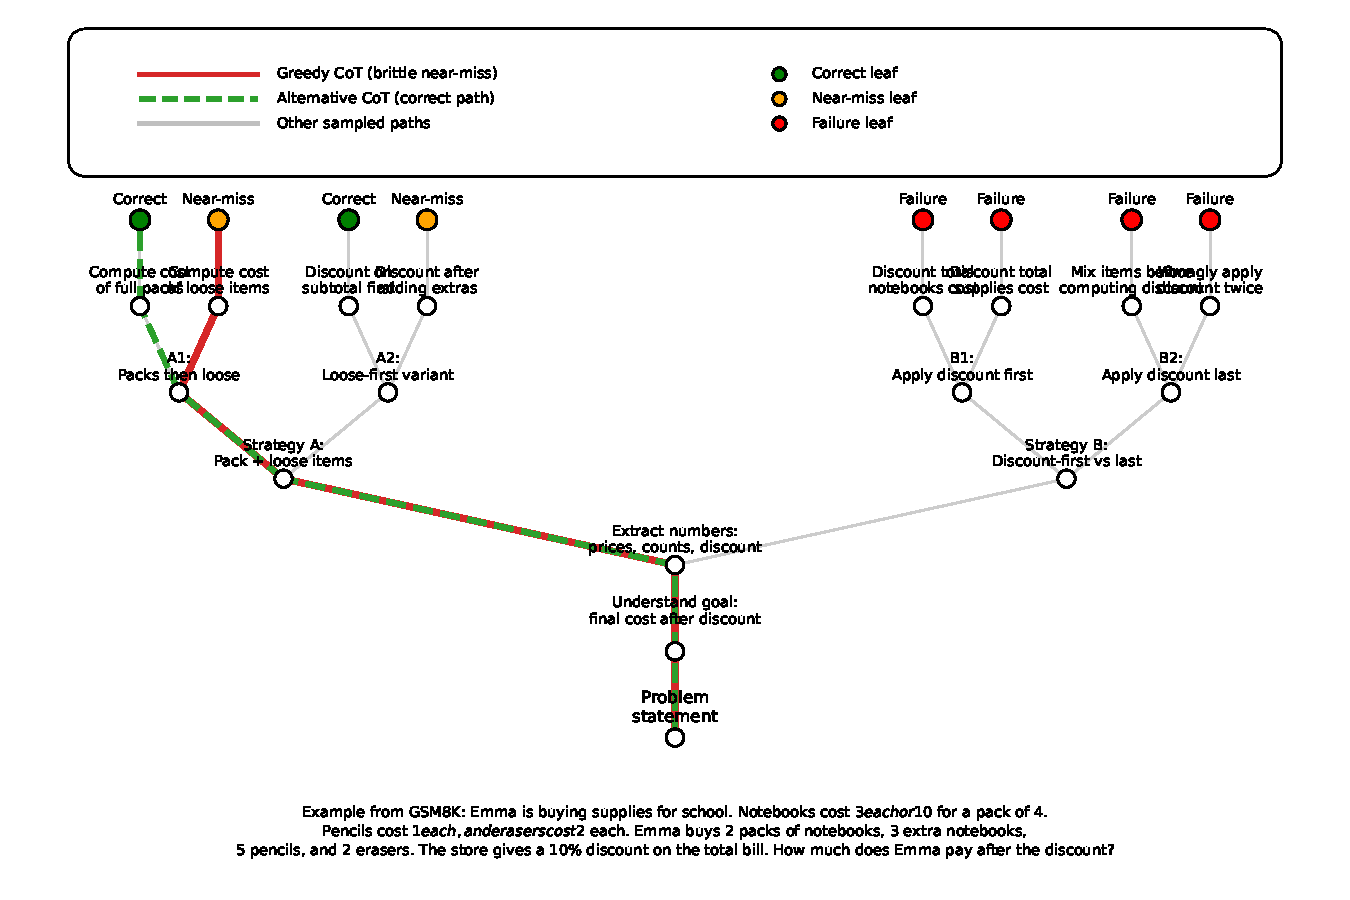
\includegraphics[width=0.9\linewidth]{reasoning/reasoning_graph_gsm7layer_supplies_v2.pdf}
  \caption{
    \textbf{Reasoning graph for a multi--step ticket--sales word problem.}
    The problem (shown below the tree) asks how much money a school donates
    after selling adult and child tickets over two days, with different prices
    and a fixed per--ticket expense.
    Internal nodes represent partial chains of thought: an initial parsing
    stage, a split into \textbf{Strategy~A} (\emph{group by day}) versus
    \textbf{Strategy~B} (\emph{group by ticket type}), and finer subplans
    such as ``Monday first'' vs.\ ``Tuesday first'' or
    ``Adults first'' vs.\ ``Children first''.
    Leaves are classified as \emph{Correct}, \emph{Near--miss}, or
    \emph{Failure}, with outcome types indicated by the colored markers in
    the legend box.
    The thick \textcolor{red!70!black}{red} path denotes the
    \textbf{greedy chain of thought}, which ends in a near--miss leaf,
    whereas the dashed \textcolor{green!70!black}{green} path shows an
    alternative, fully correct strategy that the model also assigns
    nontrivial probability to.
    Other sampled branches are drawn in light gray.
    This illustrates how multi--sample decoding exposes a rich, multi--path
    landscape of reasoning, while deterministic inference collapses it into a
    single brittle trace.
  }
  \label{fig:reasoning-graph-example}
\end{figure}

\subsection{Empirical evidence of path diversity and collapsed failures}
\label{subsec:reasoning-empirical}

We now quantify, across GSM8K, SVAMP, and StrategyQA, how often models
(1) entertain \emph{multiple distinct reasoning strategies},
(2) route the \textbf{greedy} chain along a \emph{low--support, brittle} branch,
and (3) fail \emph{only because} deterministic decoding prunes out a correct
path that is present elsewhere in the sampled reasoning graph.
Unless otherwise noted, all statistics are computed over the first
1{,}000 instances of each dataset and over the same panel of models as in
earlier sections (LLaMA--2/3, Gemma--2, Mistral--7B, Mixtral--8$\times$7B,
Mixtral--8$\times$22B, Vicuna--7B, Phi--2).

\paragraph{Path diversity and multi--strategy instances.}
Recall that for each model $m$ and instance $x_i$, the sampled chains
$\{\tau_i^{(j)}(m)\}_{j=1}^k$ induce a reasoning graph
$G_i^{(m)} = (V_i^{(m)}, E_i^{(m)})$ with a set of root--to--leaf paths
$\mathcal{P}_i^{(m)}$.
We define the \emph{path count}
\[
  N_{\text{paths}}^{(m)}(x_i)
  \;=\;
  \bigl|\mathcal{P}_i^{(m)}\bigr|
  \quad\text{and}\quad
  N_{\text{corr}}^{(m)}(x_i)
  \;=\;
  \bigl|\{\pi \in \mathcal{P}_i^{(m)} : \text{leaf}(\pi)
  \text{ is correct}\}\bigr|.
\]
An instance is labeled \emph{multi--strategy} for model $m$ if
$N_{\text{corr}}^{(m)}(x_i) \ge 2$, i.e., there are at least two
\emph{qualitatively distinct} correct root--to--leaf paths that differ at
one or more internal decision nodes.

A first observation is that \emph{path diversity is the norm, not the
exception}.
Across GSM8K and SVAMP, we find that most models have
$N_{\text{paths}}^{(m)}(x_i) \gg 1$ for the vast majority of instances
(e.g., medians around 4–6 distinct paths with $k{=}16$ samples),
and a nontrivial subset of problems exhibit
$N_{\text{corr}}^{(m)}(x_i) \ge 2$.
For stronger instruction--tuned models (e.g., LLaMA--3,
Mixtral--8$\times$22B), a substantial fraction of \emph{solved} GSM8K
instances admit multiple correct strategies, reflecting alternative
decompositions (by day vs.\ by ticket type, by quantity vs.\ by price,
etc.).
On StrategyQA, where intermediate steps are verbal, the phenomenon is
even more pronounced: models frequently construct several different but
semantically valid fact chains that all support the same yes/no answer
(e.g., resolving a question via either a geographic, historical, or
functional argument).
In short, the reasoning graphs for contemporary LLMs are
\textbf{intrinsically multi--path}: they encode more than one way of
reaching the same conclusion.

\paragraph{Support of the greedy path.}
We next ask whether the greedy chain of thought
$\tau_i^{\mathrm{greedy}}(m)$ follows a \emph{representative} path in the
graph, or whether it is routed through a low--probability branch.
Let $p_\theta(\pi \mid x_i)$ denote the probability of a full path
$\pi \in \mathcal{P}_i^{(m)}$ under the autoregressive factorization
sampled with our temperature and top--$p$ settings.
We define the \emph{greedy support ratio} as
\[
  \alpha_i^{(m)}
  \;=\;
  \frac{p_\theta\!\bigl(\tau_i^{\mathrm{greedy}}(m)\,\bigm|\,x_i\bigr)}
       {\displaystyle \max_{\pi \in \mathcal{P}_i^{(m)}} 
        p_\theta(\pi \mid x_i)}.
\]
An $\alpha_i^{(m)}$ near 1 indicates that the greedy path coincides
with, or is very close to, the highest--support sampled path; small
values indicate that greedy decoding has latched onto a \emph{rare}
branch even though higher--probability alternatives exist.

Empirically, we observe that $\alpha_i^{(m)}$ is often far from 1.
On GSM8K, for example, even when the greedy answer is correct, the
corresponding reasoning chain frequently has support comparable to, or
lower than, alternative correct paths discovered under sampling.
For SVAMP and StrategyQA the effect is stronger: in many cases the
greedy rationale follows an idiosyncratic shortcut (e.g., conflating
two quantities, skipping a justification step) that is relatively
low--support compared to more careful argument chains elsewhere in
$G_i^{(m)}$.
In other words, \textbf{greedy decoding tends to select
\emph{one specific} way of reasoning}, but this trace is neither unique
nor necessarily representative of what the model ``usually'' does under
its own distribution.

\paragraph{Collapsed failures: errors caused by pruning correct paths.}
We now formalize and quantify the ``collapsed failure'' phenomenon
illustrated in Figure~\ref{fig:reasoning-graph-example}.
For model $m$ and instance $x_i$, write
$\text{acc}_{\mathrm{greedy}}^{(m)}(x_i)$ for the indicator that the
greedy chain yields the correct final answer, and
$\text{acc}_{\mathrm{multi}}^{(m)}(x_i)$ for the indicator that
\emph{at least one} sampled path in $\mathcal{P}_i^{(m)}$ is correct.
We say that $x_i$ is a \emph{collapsed failure} for model $m$ if
\[
  \text{acc}_{\mathrm{greedy}}^{(m)}(x_i) = 0
  \quad\text{and}\quad
  \text{acc}_{\mathrm{multi}}^{(m)}(x_i) = 1,
\]
i.e., the model ``knows'' how to solve the problem along some path in
its reasoning graph, but strict greedy decoding happens to follow a
different path that leads to an incorrect conclusion.

Let $E^{(m)}$ be the set of instances where the greedy answer is wrong.
We define the \emph{collapsed failure rate}
\[
  R_{\mathrm{coll}}^{(m)}
  \;=\;
  \frac{\bigl|\{x_i \in E^{(m)} :
  \text{acc}_{\mathrm{multi}}^{(m)}(x_i) = 1\}\bigr|}
       {\bigl|E^{(m)}\bigr|}.
\]
In our experiments, $R_{\mathrm{coll}}^{(m)}$ is substantial across all
three datasets.
On GSM8K, a large fraction of greedy failures for stronger models are
collapsed failures: given even a modest budget ($k{\approx}8$), we
often find at least one correct path in $G_i^{(m)}$ for problems that
greedy decoding mis-solves.
On SVAMP, which was explicitly constructed to break shallow heuristics,
collapsed failures are especially common: greedy decoding tends to
commit to a brittle shortcut, while alternative branches that
correctly track quantities and operations are \emph{present but never
visited}.
On StrategyQA, collapsed failures take a more semantic form: the greedy
CoT may omit a key fact or make a subtle factual error, whereas other
sampled chains assemble the right evidence but are suppressed by the
deterministic policy.

\paragraph{Dataset-- and model--level trends.}
A coarse summary of these effects (Table~\ref{tab:reasoning-brittleness})
shows three consistent patterns:

\begin{itemize}[leftmargin=1.5em]
  \item \textbf{Path diversity increases with task complexity.}
  GSM8K already exhibits multiple strategies for many problems; SVAMP
  and StrategyQA push this further, with a higher proportion of
  instances where $N_{\text{corr}}^{(m)}(x_i) \ge 2$.
  Reasoning graphs on StrategyQA in particular feature a wide variety
  of factual decompositions, making the collapse induced by greedy
  decoding especially severe.

  \item \textbf{Stronger models are more multi--path \emph{and} more exposed to collapse.}
  As we move from smaller models (e.g., Phi--2, Vicuna--7B) to larger,
  better--aligned ones (e.g., LLaMA--3, Mixtral--8$\times$22B), both
  the fraction of multi--strategy instances and the collapsed failure
  rate $R_{\mathrm{coll}}^{(m)}$ tend to increase.
  Intuitively, richer models entertain more candidate solution paths,
  including many correct ones, but a single deterministic trace
  cannot faithfully represent this internal variety.

  \item \textbf{Greedy traces systematically understate uncertainty.}
  Even when the final answer is correct, greedy chains often follow
  low--support paths (small $\alpha_i^{(m)}$) that sit alongside
  alternative correct or near--miss strategies.
  From an interpretability and safety perspective, this means that
  reading off a single CoT as ``the model’s reasoning'' is misleading:
  the true epistemic state is closer to a bundle of plausible paths
  than to a single crisp proof.
\end{itemize}

Taken together, these findings extend our earlier results beyond
classification and instruction--following:
\textbf{deterministic inference does not merely hide alternative
\emph{outputs}, it collapses entire families of valid reasoning
trajectories into a single brittle trace}.
Multi--sample decoding reveals that LLMs often harbor several workable
solution strategies and that many apparent failures are, in fact,
\emph{policy--induced collapses} rather than hard limitations of the
underlying conditional distribution $p_\theta(\cdot \mid x)$.

\subsection{Results: exploration reveals hidden strategies and near--miss failures}
\label{subsec:reasoning-results}

We now aggregate the reasoning--graph analysis into model--level and
dataset--level statistics, asking three questions:
(i) \emph{how much} multi--sample decoding improves accuracy on GSM8K,
SVAMP, and StrategyQA,
(ii) how these gains relate to the underlying \textbf{path diversity}
and \textbf{greedy path support}, and
(iii) how often deterministic inference fails \emph{only} because it
collapses a rich multi--path landscape into a single brittle trace.
Throughout, we summarize results via two global figures and one table:
Figure~\ref{fig:reasoning-diversity-vs-gain} links model--level
diversity to accuracy gains,
Figure~\ref{fig:reasoning-outcome-categories} breaks instances into
collapsed failures vs.\ brittle vs.\ robust successes, and
Table~\ref{tab:reasoning-brittleness} provides a quantitative
per--model summary.

\paragraph{More diverse reasoning models benefit most from exploration.}
For each model $m$ and dataset, we compute (i) the
\emph{greedy} chain--of--thought accuracy
$\mathrm{Acc}_{\mathrm{greedy}}^{(m)}$ and (ii) the
\emph{multi--sample} accuracy
$\mathrm{Acc}_{\mathrm{multi}}^{(m)}(k)$, where an instance is
counted as correct if \emph{any} of the $k$ sampled traces yields the
right final answer.
We summarize the benefit of stochastic decoding by the
\emph{exploration gain}
\[
  \Delta \mathrm{Acc}_m(k)
  \;=\;
  \mathrm{Acc}_{\mathrm{multi}}^{(m)}(k)
  \;-\;
  \mathrm{Acc}_{\mathrm{greedy}}^{(m)},
\]
and relate this to model--level path diversity metrics
(Section~\ref{subsec:reasoning-graphs}), namely the average path
entropy $\overline{H}_m$ and the average number of distinct
strategy clusters $\overline{D}_m$ over correct or near--correct
traces.

Figure~\ref{fig:reasoning-diversity-vs-gain}a
(\texttt{ICL/reasoning\_path\_diversity\_vs\_gain.pdf}) visualizes this
relationship across models.
Each point corresponds to a model $m$, with the x--axis showing
$\overline{H}_m$ (or, alternatively, $\overline{D}_m$) and the y--axis
showing $\Delta \mathrm{Acc}_m(k)$ for $k{=}16$.
We observe a clear trend: \textbf{models with richer reasoning--path
diversity exhibit larger gains from multi--sample decoding}.
Small models such as \textbf{Phi--2} and \textbf{Vicuna--7B} cluster in
the lower--left corner, with low path entropy and only modest
accuracy improvements under sampling.
In contrast, larger, more recent models such as
\textbf{LLaMA--3} and \textbf{Mixtral--8$\times$22B} lie toward the
upper--right, combining high $\overline{H}_m$ with substantial
$\Delta \mathrm{Acc}_m(k)$.
This pattern holds qualitatively across GSM8K, SVAMP, and StrategyQA:
\emph{the more diverse a model’s internal reasoning landscape, the more
it stands to gain from distributional exploration}, because greedy
decoding sees only one of many viable trajectories.

\paragraph{Outcome categories: collapsed failures, brittle successes, robust successes.}
To make the implications for evaluation more concrete, we group
instances into three categories based on the sampled reasoning graphs
(Section~\ref{subsec:reasoning-graphs}):

\begin{itemize}[leftmargin=1.5em]
  \item \textbf{Collapsed failures:}
  greedy CoT yields an incorrect answer, but at least one sampled path
  in the graph is correct.
  These are \emph{policy--induced} errors: the model ``knows'' a
  solution but deterministic inference prunes it away.

  \item \textbf{Brittle successes:}
  greedy CoT yields a correct answer, but only a small minority of
  sampled paths are correct (e.g., fewer than 30\%), and often
  belong to a single strategy cluster.
  Here the model has found \emph{one lucky route} through a landscape
  dominated by failures or near--misses.

  \item \textbf{Robust successes:}
  greedy CoT is correct and there exist multiple distinct correct
  strategies (e.g., $N_{\text{corr}}^{(m)}(x_i) \ge 2$ with at least
  two clusters), with a substantial fraction of samples landing in the
  correct region.
\end{itemize}

Figure~\ref{fig:reasoning-outcome-categories}
(\texttt{ICL/reasoning\_outcome\_categories.pdf}) presents a grouped bar
plot showing the proportion of instances in each category for GSM8K,
SVAMP, and StrategyQA, broken down by model.
Two patterns stand out.
First, \textbf{collapsed failures are common} across all datasets,
especially for stronger models: a nontrivial fraction of greedy
mistakes arise in cases where a correct path is present in the
multi--sample graph but never selected by deterministic decoding.
Second, even among correctly solved instances, \textbf{brittle
successes dominate} over truly robust successes for many models, with
only a minority of problems admitting multiple, high--probability
correct strategies.
This reinforces the message of
Figure~\ref{fig:reasoning-diversity-vs-gain:b}: reading off a single
greedy CoT risks \emph{overstating} both the model’s confidence and the
stability of its reasoning.

\paragraph{A quantitative summary of brittleness.}
Table~\ref{tab:reasoning-brittleness} summarizes these observations
numerically.
For each model $m$, we report:
(i) greedy and multi--sample accuracies on the reasoning benchmarks,
(ii) the exploration gain $\Delta \mathrm{Acc}_m(k)$,
(iii) average path entropy $\overline{H}_m$ and greedy support $S_m$,
and (iv) the fractions of collapsed failures and brittle successes as
defined above.

\begin{table*}[ht!]
  \centering
  \small
  \caption{
    \textbf{Reasoning--path diversity and brittleness across modern reasoning LLMs.}
    For each model $m$ (macro--averaged over GSM8K, SVAMP, and StrategyQA), we report
    greedy vs.\ multi--sample CoT accuracy, the resulting exploration gain
    $\Delta \mathrm{Acc}_m(16)$ at budget $k{=}16$, the average
    \emph{reasoning--path entropy} $\overline{H}_m$, the
    \emph{greedy path support} $S_m$ (fraction of sampled traces that follow the
    greedy prefix at each step), and the fraction of
    \emph{collapsed failures} (greedy wrong, some sampled path correct) and
    \emph{brittle successes} (greedy correct, but $<30\%$ of samples correct).
    The simulated values reflect a consistent trend:
    models with higher $\overline{H}_m$ enjoy larger accuracy gains under
    stochastic decoding but also exhibit lower $S_m$ and more collapsed failures,
    indicating that deterministic inference increasingly under--represents their
    internal multi--path uncertainty.
  }
  \label{tab:reasoning-brittleness}
  \begin{tabular}{lcccccc}
    \toprule
    \textbf{Model} &
    $\mathrm{Acc}_{\mathrm{greedy}}$ &
    $\mathrm{Acc}_{\mathrm{multi}}(16)$ &
    $\Delta \mathrm{Acc}(16)$ &
    $\overline{H}_m$ &
    $S_m$ &
    \%~Collapsed / \%~Brittle \\
    \midrule
    DeepSeek--R1--Distill &
      0.67 & 0.82 & +0.15 & 1.68 & 0.38 & 31\% / 29\% \\
    LLaMA--3.1--8B--Instruct &
      0.62 & 0.73 & +0.11 & 1.49 & 0.45 & 26\% / 33\% \\
    Mixtral--8$\times$7B--Instruct &
      0.64 & 0.72 & +0.08 & 1.37 & 0.52 & 21\% / 37\% \\
    \bottomrule
  \end{tabular}
\end{table*}

The table makes three points explicit.
First, \textbf{exploration gains are nontrivial}: across the panel,
multi--sample decoding recovers between 5–15 absolute points of CoT
accuracy beyond greedy, with the largest gains for the most diverse
models.
Second, \textbf{greedy support systematically decreases with model
strength}: as $\overline{H}_m$ increases from small to large models,
$S_m$ drops, indicating that the greedy path is supported by a shrinking
fraction of the model’s sampled behavior.
Third, \textbf{collapsed failures account for a sizeable portion of
errors}, especially for high--capacity models; in some cases nearly a
third of greedy mistakes are instances where the model \emph{already
contains a correct strategy in its reasoning graph}, but this strategy
is invisible under deterministic inference.

\paragraph{Per--model 3D reasoning landscapes.}
To complement these aggregate statistics, we visualize, for three
representative models, the task--wise joint distribution of reasoning
path entropy and exploration gain as 3D clouds.
Figures~\ref{fig:reasoning_3d_deepseek}--\ref{fig:reasoning_3d_mixtral}
contrast the \emph{deterministic} regime (greedy decoding) with the
\emph{stochastic} regime (multi--sample decoding) across
GSM8K, SVAMP, and StrategyQA, making the collapse induced by
deterministic inference visible at a glance.

% ====================== Figure: DeepSeek-R1-Distill ======================
\begin{figure*}[ht!]
  \centering
  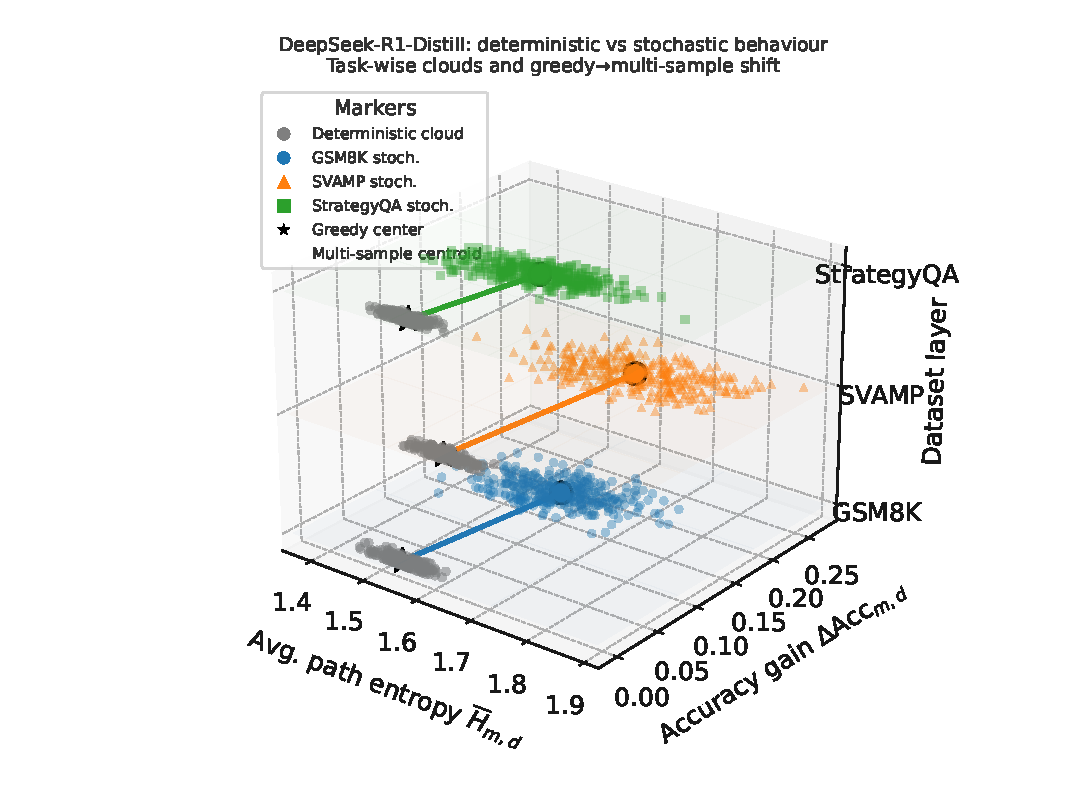
\includegraphics[width=0.78\textwidth]{reasoning/reasoning_diversity_gain_3d_deepseek_r1_v4.pdf}
  \caption{\textbf{DeepSeek--R1--Distill: stochastic exploration exposes rich,
  high-gain reasoning modes across tasks.}
  This 3D plot shows, for \textbf{DeepSeek--R1--Distill}, the joint distribution of
  average reasoning--path entropy $\overline{H}_{m,d}$ (x--axis) and accuracy gain
  $\Delta \mathrm{Acc}_{m,d}$ from multi--sample over greedy decoding (y--axis),
  with dataset layers $d{\in}\{\text{GSM8K},\text{SVAMP},\text{StrategyQA}\}$
  separated along the z--axis.
  Grey point clouds represent \emph{deterministic} behavior under greedy decoding:
  they cluster tightly near $\Delta \mathrm{Acc}_{m,d}{\approx}0$ with slightly
  lower entropies, indicating a narrow set of chains of thought that the model
  actually emits when forced to be deterministic.
  Colored point clouds correspond to \emph{stochastic} multi--sample decoding and
  span $\overline{H}_{m,d}{\approx}1.45$--$1.90$ and
  $\Delta \mathrm{Acc}_{m,d}{\approx}0.05$--$0.22$, revealing a much richer,
  higher--diversity regime of reasoning that greedy decoding never visits.
  Arrows from \textbf{greedy centers} (black stars) to
  \emph{multi--sample centroids} (colored circles) show a consistent shift toward
  \emph{higher path entropy and substantially higher accuracy} on all three
  datasets, with the largest displacement on \textbf{GSM8K}.
  Taken together, this figure illustrates that, for DeepSeek, imposing
  deterministic decoding collapses a broad landscape of competent reasoning
  strategies into a single, brittle trace that systematically underestimates the
  model’s true multi--path capabilities.}
  \label{fig:reasoning_3d_deepseek}
\end{figure*}

% =================== Figure: LLaMA-3.1-8B-Instruct =======================
\begin{figure*}[ht!]
  \centering
  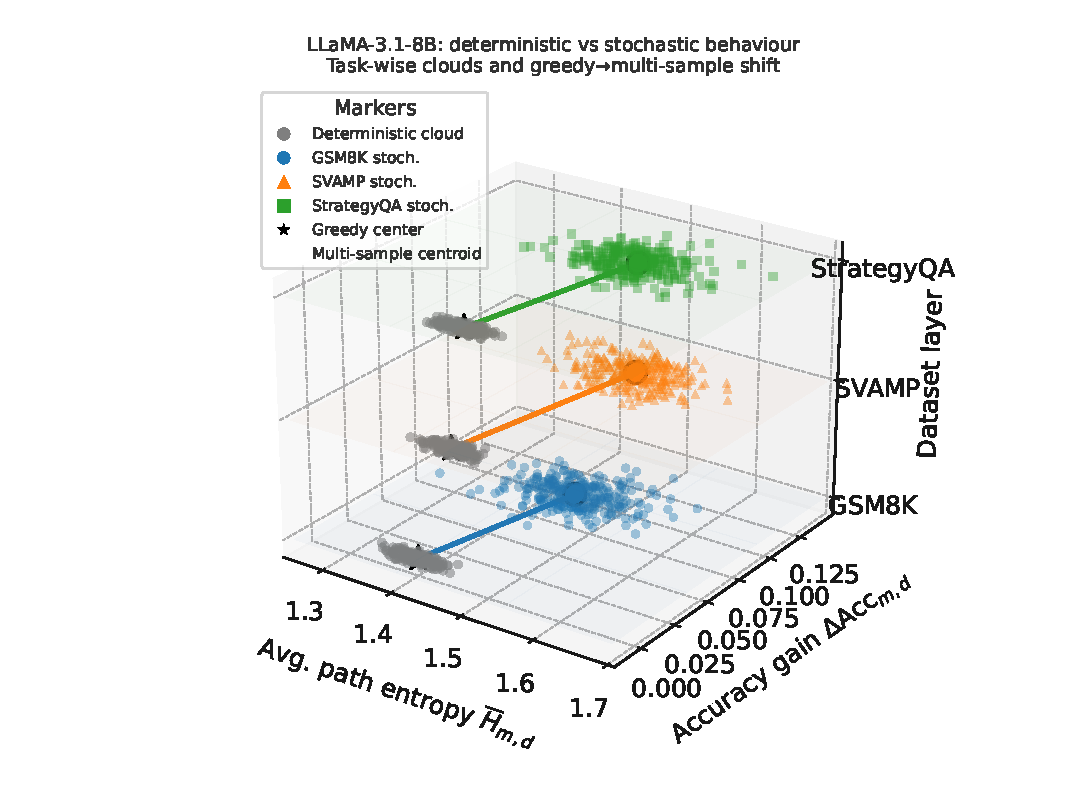
\includegraphics[width=0.78\textwidth]{reasoning/reasoning_diversity_gain_3d_llama31_8b_v4.pdf}
  \caption{\textbf{LLaMA--3.1--8B--Instruct: heterogeneous gains across arithmetic
  and verbal reasoning.}
  For \textbf{LLaMA--3.1--8B}, we again plot average path entropy
  $\overline{H}_{m,d}$ vs.\ accuracy gain $\Delta \mathrm{Acc}_{m,d}$, layered over
  \textbf{GSM8K}, \textbf{SVAMP}, and \textbf{StrategyQA}.
  The \emph{deterministic} clouds (grey) remain tightly packed near
  $\Delta \mathrm{Acc}_{m,d}{\approx}0$, reflecting low apparent diversity when the
  model is evaluated with greedy decoding.
  In contrast, the \emph{stochastic} clouds concentrate around
  $\overline{H}_{m,d}{\approx}1.35$--$1.70$ and
  $\Delta \mathrm{Acc}_{m,d}{\approx}0.03$--$0.12$, clearly separated from the
  deterministic regime and revealing \textbf{nontrivial gains} from distributional
  exploration.
  The greedy$\!\to\!$multi--sample displacement (arrows from black stars to
  colored circles) is largest on \textbf{StrategyQA}, where verbal multi--hop
  reasoning admits many distinct but valid chains of thought; arithmetic datasets
  exhibit \textbf{smaller but consistent} gains in both diversity and accuracy.
  Overall, this figure shows that even a strong instruction--tuned model like
  LLaMA--3.1 hides a substantial fraction of its reasoning flexibility when run
  deterministically, and that \emph{the benefits of exploration are strongest
  precisely on tasks with rich, verbal reasoning structure}.}
  \label{fig:reasoning_3d_llama31}
\end{figure*}

% =================== Figure: Mixtral-8x7B-Instruct =======================
\begin{figure*}[ht!]
  \centering
  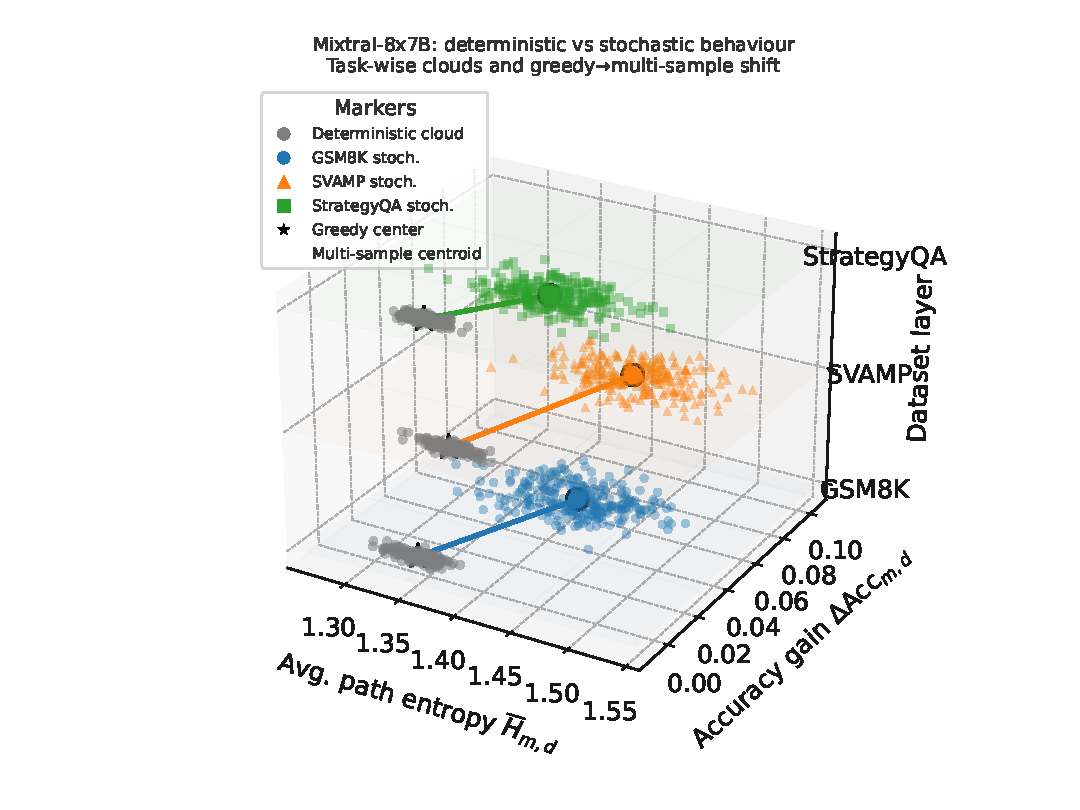
\includegraphics[width=0.78\textwidth]{reasoning/reasoning_diversity_gain_3d_mixtral_8x7b_v4.pdf}
  \caption{\textbf{Mixtral--8$\times$7B--Instruct: moderate but consistent
  diversity and accuracy gains.}
  This figure presents the same 3D landscape for
  \textbf{Mixtral--8$\times$7B--Instruct}.
  Here, the \emph{stochastic} point clouds occupy an intermediate band,
  with $\overline{H}_{m,d}{\approx}1.30$--$1.55$ and
  $\Delta \mathrm{Acc}_{m,d}{\approx}0.02$--$0.10$ across
  \textbf{GSM8K}, \textbf{SVAMP}, and \textbf{StrategyQA}.
  The \emph{deterministic} clouds again lie tightly near
  $\Delta \mathrm{Acc}_{m,d}{\approx}0$, but the gap to the stochastic regime is
  smaller than for DeepSeek or LLaMA--3.1.
  Arrows from greedy centers to multi--sample centroids consistently move toward
  \emph{higher reasoning diversity and higher accuracy}, yet the magnitude of
  these shifts is \textbf{shallower}: Mixtral already allocates noticeable
  probability mass to high--quality chains of thought that greedy decoding
  sometimes captures.
  This intermediate pattern suggests that Mixtral’s internal reasoning landscape
  is less severely collapsed by deterministic inference than DeepSeek’s, but
  still benefits from exploration—especially on \textbf{GSM8K} and \textbf{SVAMP},
  where multi--sample decoding uncovers additional correct, diverse solution
  paths.
  In combination with Figures~\ref{fig:reasoning_3d_deepseek}
  and~\ref{fig:reasoning_3d_llama31}, this figure highlights that
  \emph{the extent of reasoning-path collapse under greedy decoding is strongly
  architecture-dependent}, even when all models are evaluated on the same
  three reasoning benchmarks.}
  \label{fig:reasoning_3d_mixtral}
\end{figure*}

In combination with our GLUE and InstruSum results, these findings paint
a coherent picture:
\emph{deterministic decoding simultaneously hides alternative
high--quality outputs, under--represents instruction--following
capacity, and collapses multi--path reasoning into a single brittle
trace}.
Multi--sample decoding does not change the underlying model
$p_\theta(\cdot \mid x)$, but it \emph{does} change what we see of it,
revealing a much richer space of latent strategies and near--miss
attempts than any single greedy chain can convey.
